\documentclass[10pt, a4paper]{article}
\usepackage[T1]{fontenc}
\usepackage[left=2cm, right=2cm, top=2cm, bottom=2cm]{geometry}
\usepackage{graphicx}
\usepackage{mathtools}
\DeclareMathOperator{\arcsinh}{arcsinh}
\usepackage{amssymb}
\usepackage{wasysym} % for \astrosun and more!
\usepackage{mathrsfs} % to use \mathscr{...}
\usepackage{xcolor} % \textcolor{red}{...} & \mathcolor{red}{...}
\usepackage{hyperref} %Automatically links \label and \ref commands; Always load last
\hypersetup{
	linktocpage,
	colorlinks=true, % false: boxed links; true: colored links
	linkcolor=red, % color of internal links
	citecolor=blue, % color of links to bibliography
	filecolor=magenta, % color of file links
	urlcolor=purple, % color of external links
} % hidelinks
%----------------------------------------------------------------------
\usepackage{fancyhdr}

\pagestyle{fancy}
\fancyhf{}  % Clear all headers and footers

% Redefine section mark to include section number and title
\renewcommand{\sectionmark}[1]{%
	\markboth{Section \thesection\ #1}{}%
}

\fancyhead[L]{\nouppercase{\leftmark}}  % Header always on the left
\fancyfoot[C]{\thepage}                 % Centered page number
%----------------------------------------------------------------------
% for XeTeX
\usepackage{xeCJK}
\setCJKmainfont{GenRyuMin JP} % 源流明体
\setCJKmonofont{GenRyuMin JP} % font used in \texttt{} (just to prevent a warning)
% for LuaTeX
%\usepackage{luatexja-fontspec}
%\setmainjfont{GenRyuMin2 JP} % 源流明体
%----------------------------------------------------------------------
% to handle a large project
\usepackage{import}
%----------------------------------------------------------------------
\usepackage{indentfirst}
\setlength{\parindent}{0em} % 首行缩进
%----------------------------------------------------------------------
% horizontal line
%\noindent\rule[0.5ex]{\linewidth}{0.5pt} % horizontal line
\usepackage{dashrule}
%\noindent\hdashrule[0.5ex]{\linewidth}{0.5pt}{1mm} % horizontal dashed line
%----------------------------------------------------------------------
\usepackage[breakable]{tcolorbox} % box with color; highlight text \colorbox{yellow}{...}
\tcbset{breakable, colback=white, colframe=green!30!black, coltext=black!60!white, fonttitle=\bfseries}

\usepackage{tabularx} % LaTeX table
\usepackage{booktabs}

\usepackage{float} % appropriate way to handle figures
% example:
%\begin{figure}[H]
%	\centering
%	\includegraphics[scale=1]{figures/file-name}
%	\caption{...}
%\end{figure}
\usepackage{subcaption}
% following David Tong's convention, one should always add a caption to figures, but not to tables.
% use \vcenter{\hbox{\includegraphics[...]{...}}} to insert figures (e.g. Feynman diagrams) in equation environment.
%----------------------------------------------------------------------
\numberwithin{equation}{section}
\allowdisplaybreaks % allow page breaks inside math environments globally

\usepackage{braket}
\usepackage{cancel}

\usepackage{leftindex}
\usepackage{tensor} % how to handle indeces: https://tex.stackexchange.com/questions/11542/left-and-right-subscript-superscript
\usepackage{isotope} % e.g. \isotoe[4][2]{He} = helium-4

\usepackage{simpler-wick} % to use Wick contraction
%\usepackage[compat=1.1.0]{tikz-feynman}

% use \, in math environment
% except for texts embeded in math environment, use \ instead
%----------------------------------------------------------------------
\usepackage{orcidlink}
%----------------------------------------------------------------------
\title{\Huge \textbf{Path Integral Numerically}}
\author{Siyang Wan (万思扬)}
\date{June 2, 2025}
%----------------------------------------------------------------------
\begin{document}
	\maketitle
	
	\pdfbookmark{\contentsname}{toc} % add pdf bookmark to the ToC
	\tableofcontents
	
	\section{path integral}
	\begin{itemize}
		\item 考虑系统的 Hamiltonian 为
		\begin{equation}
			H = \frac{p^2}{2 m} + V(x),
		\end{equation}
		那么其 Lagrangian 为
		\begin{equation}
			L = \frac{m}{2} \dot{x}^2 - V(x),
		\end{equation}
		系统初态为 $\ket{\psi_0}$.
		
		\item 用 path integral 计算 $\psi(T, x) = \braket{x | e^{- i H T} | \psi_0}$, 有
		\begin{align}
			\braket{x | e^{- i H T} | \psi_0} =& \int Dx \, e^{i \int_0^T dt \, L} \notag \\
			=& \lim_{N \rightarrow \infty} \int dx_0 \, \psi_0(x_0) \int dx_{N + 1} \, \delta(x_{N + 1} - x) \notag \\
			& \int dx_1 \cdots dx_N \, \exp \Big( i \sum_{i = 0}^N \Delta t \Big( \frac{m}{2} \Big( \frac{x_{i + 1} - x_i}{\Delta t} \Big)^2 - V(x_i) \Big) \Big),
		\end{align}
		其中 $\Delta t = \frac{T}{N + 1}$.
		
		\item 数值计算中, 令
		\begin{equation}
			\begin{dcases}
				x_i = \Big( \frac{2 i}{M} - 1 \Big) L, \Delta x = \frac{2 L}{M}, i = 0, \cdots, M \\
				K_{i j} = \braket{x_i | e^{- i H \Delta t} | x_j} = \sqrt{\frac{m}{2 \pi i \Delta t}} \exp \Big( i \Big( \frac{m}{2} \frac{(x_i - x_j)^2}{\Delta t} - \Delta t V(x_i) \Big) \Big)
			\end{dcases},
		\end{equation}
		那么
		\begin{equation}
			\braket{x | e^{- i H T} | \psi_0} = \lim_{L, M, N \rightarrow \infty} (\Delta x)^{N + 1} \sum_{j = 0}^M (K^{N + 1})_{i j} \psi_0(x_j), \quad \text{with} \quad x_i = x \ll L.
		\end{equation}
	\end{itemize}
	
	\subsection{Gaussian wave packet}
	\begin{itemize}
		\item 考虑一个自由粒子, 初态为
		\begin{equation}
			\psi_0(x) = \Big( \frac{2}{\pi} \Big)^{\frac{1}{4}} e^{- x^2 + i k_0 x}, \quad \braket{k | \psi_0} = \frac{1}{(2 \pi)^{1 / 4}} e^{- \frac{1}{4} (k - k_0)^2},
		\end{equation}
		那么, 预期结果为
		\begin{equation}
			\psi(t, x) = \Big( \frac{2}{\pi} \Big)^{\frac{1}{4}} \sqrt{\frac{m}{m + 2 i t}} \exp \Big( \frac{m}{m + 2 i t} (- x^2 + i k_0 x) - i \frac{k_0^2}{2 (m + 2 i t)} t \Big).
		\end{equation}
		
		\item 用路径积分数值计算得到的结果如下图所示 ($A = \int dx \, \rho$ 是 normalization constant):
		
		\begin{figure}[H]
			\centering
			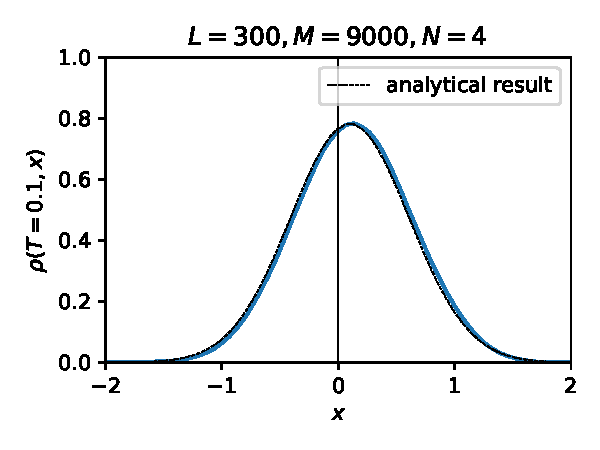
\includegraphics[scale=0.8]{figures/path integral numerically (normalized) of a free particle with initial state as a Gaussian wave packet and T=0.1 (L=300, M=9000, N=4).pdf}
			\caption{path integral numerically (normalized, $A \sim 10^{11}$) with $T = 0.1$.}
		\end{figure}
	\end{itemize}
\end{document}